\subsection{Identification of GW sources}
It is important to note that, though we present predictions for the detection rates of specific DCO types, the nature of the source may not be immediately apparent from the gravitational wave signal.

\subsubsection{Distinguishing from WDWD population}\label{sec:WDWD_distinguish}
The population of Galactic WDWDs detectable with LISA will be several orders of magnitude larger than the more massive DCOs on which we focus in this paper \citep[e.g.][]{Korol+2017}. It is therefore imperative that we consider how to distinguish NS and BH binaries from this much more numerous population of sources.

The simplest way to check whether a source is a WDWD is to check its chirp mass. The mass of a non-rotating white dwarf cannot be larger than the Chandrasekhar limit of $1.44 \unit{M_\odot}$ \citep{Chandrasekhar+1931}, so we can take the maximum chirp mass of a WDWD to be $\sim 1.25 \unit{M_{\odot}}$. Therefore, any DCO with a chirp mass that satisfies $\mathcal{M}_c > 1.25 \unit{M_{\odot}} + 2 \Delta \mathcal{M}_c$ must not be a WDWD. We find that for a 4(10)-year LISA mission, 17(23)\% of BHBHs, 20(24)\% of BHNSs and 2.4(2.5)\% of NSNSs satisfy this condition. As one would expect, this method is not particularly effective for NSNSs since their average chirp mass, $1.17 \unit{M_\odot}$, is below the Chandrasekhar limit.

Another indicator that the source is not a WDWD would be that it is eccentric. WDWDs formed in the disc are thought to be formed through isolated binary formation and have little to no eccentricity \citep[e.g.][]{Nelemans+2001}. Therefore, if any system is detected with anything other than one detectable harmonic, this implies that the system is unlikely to be a WDWD. We find that for a 4(10)-year LISA mission, 55(61)\% of BHBHs, 27(28)\% of BHNSs and 65(69)\% of NSNSs are detected with multiple harmonics. Both the absolute percentage and the improvement with an extended LISA mission is lower for the BHNSs as we find that these DCOs are less eccentric on average (see Fig.~\ref{fig:fiducial_pdf_distributions}).

However, we should also consider that eccentric WDWDs \textit{could} be formed through dynamical formation in Milky Way globular clusters \citep[e.g.][]{Willems+2007, Kremer+2018}. This means that it would not be valid to assume that eccentric binaries are not WDWDs unless they are detected in the Galactic plane. Therefore, we can use the sky localisation, scale height of the disc and distance to the source to estimate what fraction of eccentric sources can be localised to the Galactic plane. This condition can be written as $\sigma_\theta < \arcsin(z_{\rm plane} / D_L)$ or $D_L < z_{\rm plane}$, where we set the height of the Galactic plane, $z_{\rm plane}=0.95 \unit{kpc}$, to the scale height of the high-$\alpha$ disc. We apply this condition to find that the fraction of sources that are eccentric \textit{and} localised within the disc for a 4(10)-year LISA mission are 40(32)\% for BHBHs, 24(19)\% for BHNSs and 59(51)\% for NSNSs\footnote{Note that although the fractions are smaller for the 10 year mission, the \textit{absolute} number of detections is still greater. The fraction decreases because a 10 year mission detects more `marginal' sources that are just on the cusp of the detection threshold and these sources have the worst sky localisation and thus cannot be confirmed to lie within the Galactic plane.}.

Overall, combining these methods we find that for a 4(10)-year mission, LISA will detect at least \BHBHNotWDWDFour{}(\BHBHNotWDWDTen{}) BHBHs, \BHNSNotWDWDFour{}(\BHNSNotWDWDTen{}) BHNSs and \NSNSNotWDWDFour{}(\NSNSNotWDWDTen{}) NSNSs that are distinguishable from the WDWD population.

\subsubsection{Separating BHBHs, BHNSs and NSNSs}

The problem of separating the BHBH, BHNS and NSNS population can be more difficult. We can follow a similar method to the WDWDs (see Sec.~\ref{sec:WDWD_distinguish}) by applying our knowledge of the maximum mass of a neutron star. Following our fiducial assumption, we can take the maximum mass of a neutron star as $2.5 \unit{M_{\odot}}$ and thus the maximum chirp mass that a system can attain without one of the components being a black hole is $\mathcal{M}_{c} = 2.2 \unit{M_\odot}$. For a 4(10)-year LISA mission, the fraction of systems that are above or below this limit by more than $2 \Delta \mathcal{M}_c$ is 15(20)\% for BHBHs, 12(14)\% for BHNSs and 34(40)\% of NSNSs, which in terms of absolute detections is \BHBHDistinguishedFour{}(\BHBHDistinguishedTen{}) for BHBHs, \BHNSDistinguishedFour{}(\BHNSDistinguishedTen{}) for BHNSs and \NSNSDistinguishedFour{}(\NSNSDistinguishedTen{}) for NSNSs. For separating the BHBH and BHNS population one could consider the range of mass ratios that could result in the chirp mass and assume that those that are likely close to unity must be BHBHs.

Another possible solution would be the existence of electromagnetic counterparts to the gravitational wave signal. In the next section (Sec.~\ref{sec:pulsar_matching}) we consider the possibility of detecting a pulsar within a BHNS or NSNS system. This could be used to identify the type of the source, however it is unlikely that a large fraction of the population will contain pulsars that are beaming towards the Earth.

One could also consider using the eccentric or orbital frequency to separate the populations since the distributions are reasonable different for each DCO type (see Fig.~\ref{fig:fiducial_pdf_distributions}). This method would also pose a challenge as it would likely only favour one DCO type as the source of the signal rather than provide strong evidence as the chirp mass could.

\subsection{Matching LISA detections to pulsars with SKA}\label{sec:pulsar_matching}
Since the vast majority of the LISA detectable population of DCOs will not merge for many years, the main form of electromagnetic counterpart for the this population is pulsars. Therefore, for this section we focus only on BHNSs and NSNSs since no BHBH system will contain a pulsar. The joint detection of a binary pulsar with LISA and SKA would not only help to constrain the parameters of the binary, but also enable investigation of other compact object physics. A pulsar(PSR)+BH can be provide stringent tests of theories of gravity, in particular the ``No-hair theorem'' \citep{Keane+2015}. Altneratively, an ultrarelativstic PSR+NS system could be used to measure the neutron star equation of state up to an order of magnitude better than other proposed observations \citep{Kyutoku+2019, Thrane+2020}.

In this section, we perform some back-of-the-envelope calculations to order to estimate how we can use SKA to match pulsars to LISA detections.

First, we can consider how many pulsars SKA is likely to detect. \citet{Keane+2015} uses PSRPOPPy \citep{Bates+2014} to simulate the Milky Way pulsar population. They find that for SKA-1, approximately $10000$ pulsars will be discovered. The second phase of SKA, which should also have been approved and be in operation by the time of the LISA mission, would yield a total of $35000$-$41000$ pulsars \citep{Keane+2015}, where we use the average, $38000$, in further estimates below. Moreover, we are only interested in pulsars that are part of a binary system. We can estimate this pulsar binary fraction as the fraction of known pulsars that are in binaries using the ATNF Pulsar Catalogue\footnote{\url{https://www.atnf.csiro.au/research/pulsar/psrcat}} \citep{Manchester+2005}. $290$ of the $2872$ currently known pulsars are in binary systems and thus we can estimate the binary fraction of pulsars as $10\%$.

Next, we can find the total number of pulsars SKA will detect in a patch on the sky. The total sky area that the SKA mission covers is approximately $7200 \unit{deg^2}$, which is calculated by integrating over the sky for all Galactic longitudes and Galactic latitudes limited to $\abs{b} < 10^\circ$, which are the limits on SKA-mid \citep{Keane+2015}. If we assume that the pulsars are found uniformly across the sky, this means that roughly $0.14$ and $0.49$-$0.57$ binary pulsars are expected per square degree for SKA-1 and SKA-2 respectively. Note that the assumption assumption of a uniform distribution is not realistic as pulsars will tend to be far more concentrated in the Galactic centre but we use it to provide an upper bound on these estimates.

Alternatively, we could write that we expect a single pulsar per $7.2 \unit{deg^2}$ and $2.1$-$1.8 \unit{deg^2}$ for SKA-1 and SKA-2 respectively, which corresponds to angular resolutions of $\sigma_\theta = 1.51^\circ$ and $\sigma_\theta = 0.82$-$0.76^\circ$. Given these estimates, and by considering the last panel of Fig.~\ref{fig:fiducial_pdf_distributions}, approximately $10$ and $6$ (for SKA-1 and SKA-2) DCOs containing NSs will be localised well enough such that, \textit{if} the NS is a pulsar, SKA can unambiguously match it to the radio signal.

If there is more than one pulsar in the region given by the LISA sky localisation, one can compare the measured parameters of the system in LISA and SKA. Both SKA and LISA will measure the orbital frequency to high precision, as well as the time derivative of the frequency and chirp mass to a lesser precision, of each of these systems. Therefore, one could perform a targetted search with SKA that checks the sky location given by LISA and only looking for binary pulsars with orbital frequencies within the errors. If there was \textit{still} more than one possible pulsar one could then also check against the chirp mass. In this way, it would still be possible to get a joint detection between SKA and LISA even when the sky area implied by the LISA detection contains more than one pulsar.

In order to assess the efficacy of this method, we would need to know the probability that two random binary pulsars would have orbital frequencies and chirp masses close enough that one could not tell which pulsar matches the LISA detection. This would require simulating the SKA population of pulsars with a code such as PSRPOPPy to find the frequency and chirp mass distribution and thus is beyond the scope of this paper. However, the uncertainty on the orbital frequency of a binary on the detection threshold ($\rho = 7$) for a 4-year LISA mission is $2.5 \times 10^{-9} \unit{Hz}$ and $1.0 \times 10^{-9} \unit{Hz}$ for a 10-year mission (calculated using Eq.~\ref{eq:f_orb_unc}). Therefore, we expect that SKA could likely isolate the correct binary pulsar to match to a LISA detection even when several are present in the sky localisation region.

\subsection{Assessing the impact of Milky Way model choices}
The model that we use for the Milky Way adds several layers of complexity, accounting for the inside-out growth of the thin disc, using empirically informed star formation histories that are a function of time and assigning metallicities based on the position and age of binaries. In this section, we repeat our main analysis but instead apply a simpler model for the Milky Way in order to assess the effect of these added features. For this purpose, we use model for the Milky Way used in \citet{Breivik+2020} as this is representative of the models used in most previous works.

Their model can be summarised as follows: the Milky Way is assumed to comprise of three components, a thin disc, a thick disc and a bulge. The spatial distributions and relative masses for these components are given in \citet{McMillan+2011}. \citet{Breivik+2020} assume constant star formation over 10 Gyr for the thin disc, a 1 Gyr burst of star formation 11 Gyr ago for the thick disc and a 1 Gyr burst of star formation 10 Gyr ago for the bulge. A major difference is that only two metallicities are used and they are assigned independent of age or position. Binaries formed in the thin disc and bulge are assumed to have a metallicity of $Z = 0.02$ and those formed in the thick disc are assumed to have $Z = 0.003$.

We show this model in Fig.~\ref{fig:simple_mw} in the same form as Fig.~\ref{fig:galaxy_schematic} for ease of comparison between our models. The two main differences we can see in these plots are that the \citet{Breivik+2020} model is more centrally concentrated and only has two fixed metallicity populations.
%In addition, though it can't be seen in these plots, the simpler prescriptions for the star formation histories mean that the overall star formation history is highly discontinuous at $\tau = 9 \unit{Gyr}$ and significantly more star formation occurs from $\tau = 9 \unit{Gyr}$ to $\tau = 11 \unit{Gyr}$.

\begin{figure}[t]
    \centering
    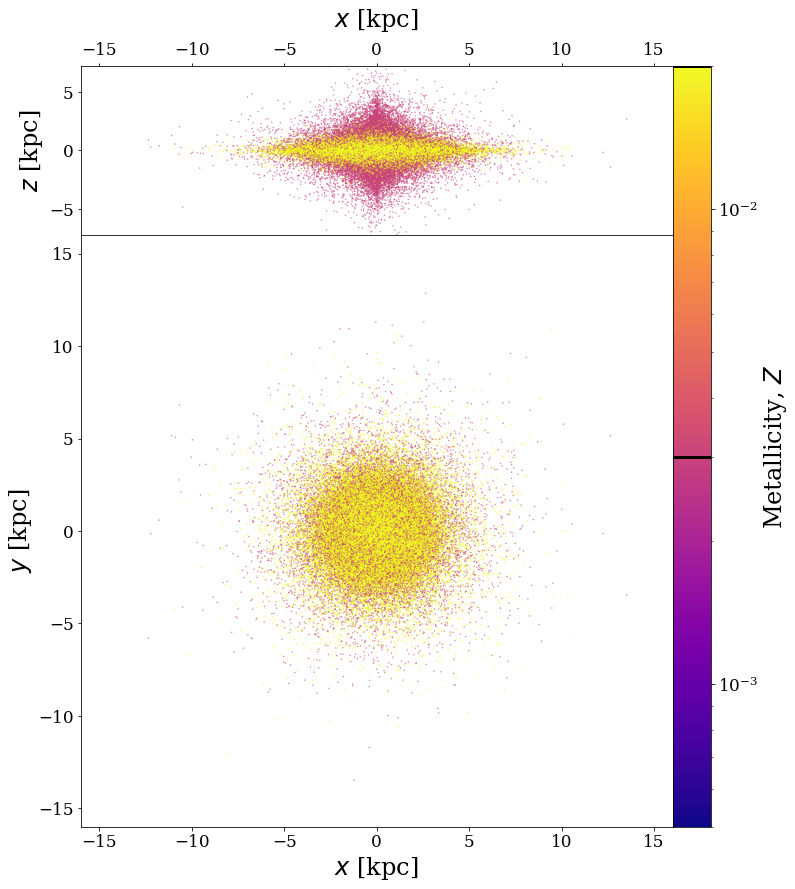
\includegraphics[width=\columnwidth]{../figures/random_simple_galaxy.png}
    \caption{As Fig.~\ref{fig:galaxy_schematic} (right panel), but for the Milky Way model used in \citet{Breivik+2020}.}
    \label{fig:simple_mw}
\end{figure}

We find that when applying this simpler Milky Way model and our fiducial physics assumptions (model \modFid{}), the expected number of detections for BHBHs, BHNSs and NSNSs for a 4-year LISA mission is $39$, $39$ and $14$ respectively. Thus the BHBH and BHNS detection rates are only marginally increased from our main findings, but the NSNS detection is overestimated by nearly a factor of 2.

Moreover, the distribution of parameters within the population, particularly the mass distributions, are notably disparate. By using only two fixed metallicity populations, unphysical artifacts are introduced into distribution of DCO masses (Kummer at al. (in prep)). For example, in Fig.~\ref{fig:bh_mass_simple_mw}, we show the black hole mass distribution produced by the simulation using the simple Milky Way model. Despite the fact that these KDEs use the same bandwidth as Fig.~\ref{fig:fiducial_pdf_distributions}, the distributions show many more sharp transitions, which is a result of pileups occurring at specific masses for specific metallicities. Moreover, the lack of lower metallicities systems means that higher mass systems are not formed and so we see the distributions do not include a high mass tail such as in our fiducial results.

The unphysical artifacts present in the mass distributions can have far-reaching effects since the masses of DCOs affect most other parameters. The inspiral time and SNR are directly dependent on the mass, whilst the uncertainty estimates depend on the SNR. This means that the artifacts can affect the predictions for most distributions of LISA detectable populations.

Overall, we find that previous studies that use Milky Way models analogous to this simpler model may significantly overestimate the LISA NSNS detection rate as well as contain unphysical artifacts in their parameter distributions.

\begin{figure}[h]
    \centering
    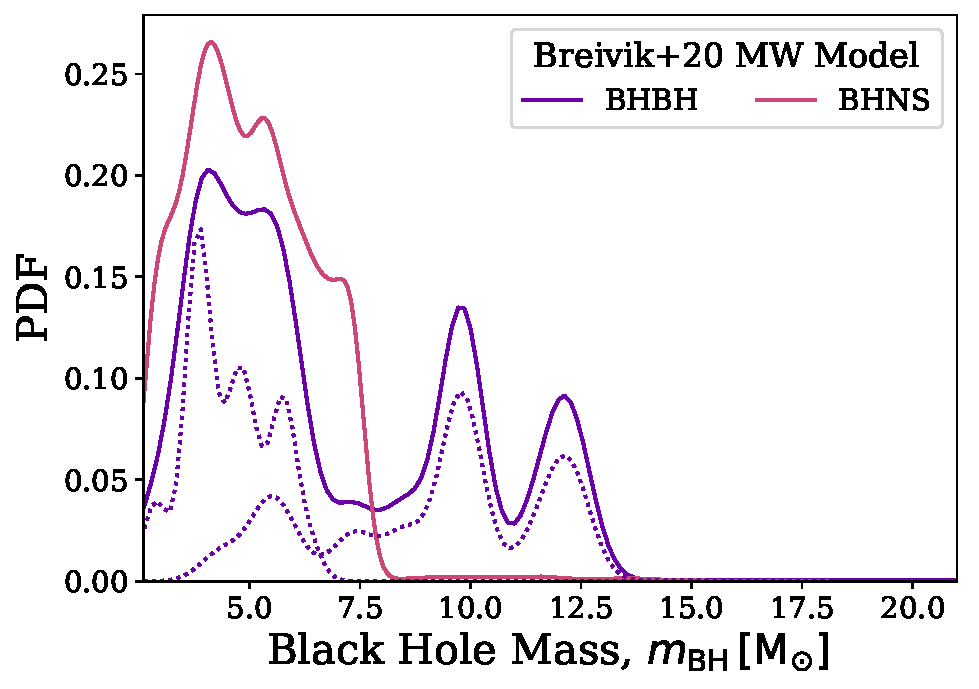
\includegraphics[width=\columnwidth]{../figures/BH_mass_dist_simple_mw.pdf}
    \caption{As Fig.~\ref{fig:fiducial_pdf_distributions} (top left panel), but for the Milky Way model used in \citet{Breivik+2020}.}
    \label{fig:bh_mass_simple_mw}
\end{figure}

\subsection{Caveats}\label{sec:caveats}
\textit{Population synthesis limitations:} As with any study involving a population synthesis code, our results rely on uncertain stellar physics and the use of approximate fitting formulae. We cannot use detailed stellar evolution codes to produce such a large sample of DCOs in a reasonable amount of time. Therefore COMPAS uses fitting formulae and approximate prescriptions based on (sometimes limited) grids of detailed models to describe the evolution of binary stars. This means that some of the finer points of evolution may be approximated but generally the final product of the stars on a population as a whole is reasonably close to the true result. In addition, much of the underlying physics is uncertain, such as the common envelope evolution and mass transfer physics. We attempt to understand the importance of these assumptions by creating many different physics variations. However, it is not reasonable to change every possible parameter (especially since many parts of the code have fixed assumptions) and therefore our results are subject to the accuracy of the assumptions made within the COMPAS code.

\textit{Underlying helium star models:} One major weakness is that the \citet{Hurley+2000} fitting formulae for the evolution of helium stars are based on a grid of models from $0.3 \unit{M_{\odot}}$ to $10 \unit{M_{\odot}}$, for a single metallicity ($Z= 0.02$) and thus the formulae have no metallicity dependence and are extrapolated for higher masses. A more detailed set of models in this regime could lead to large changes in the evolution of naked helium stars, a common progenitor of DCOs, and thus affect the detection rate of DCOs.

\textit{Limited metallicity range:} Another limitation of the stellar evolution fitting formulae that COMPAS uses is that they are limited to a metallicity range of $10^{-4} \le Z \le 0.03$ and should not be extrapolated outside this region. On the scale of the Universe (more relevant for LIGO predictions), this does not usually pose a significant problem as the population is usually fairly low metallicity. However, for local GW detection in the Milky Way (based on the metallicity relation in \citet{Frankel+2018}), the metallicity distribution can extend as far as $10^{-5} \le Z \le 0.06$, with a significant fraction of formation occurs past $Z = 0.03$. Therefore, for our study we had to reassign any metallicities outside of COMPAS' range. For any metallicity below the minimum, we places it in our lowest metallicity bin. For any metallicity above the minimum we placed it uniformly randomly in one of the top 5 highest bins (since using a single bin for many binaries led to unphysical artifacts in our results).

\textit{Other formation channels:} We also note that our findings are only the result of a single formation channel (isolated binary formation). We do not consider other channels such as dynamical formation or chemically homogeneous evolution, which could increase the detection rate and alter the parameter distributions. For instance, \citet{Kremer+2018} showed that around $21$ systems could be detected in Milky Way globular clusters through dynamical formation and thus different channels can still contribute significantly to the detection rate.

\textit{Halo and globular clusters:} Moreover, our model for the Milky Way, though more extensive than many previous studies, does not consider the contributions from the Galactic halo or globular clusters. \citet{Lamberts+2018} found that the halo's contribution to the detection rate was minimal and, since the metallicity distribution of the halo is uncertain, we did not include it in our galaxy model. The impact of globular clusters would have required a more detailed look into dynamical formation that was beyond the scope of this paper but we again highlight the work of \citet{Kremer+2018} that investigated these rates.

\textit{Systemic kicks:} Another important consideration about our galaxy is that we do not include the effect of systemic kicks on the final location of the sources. This would require integrating the orbital evolution of the millions of binaries in our sample and thus was not computationally reasonable to include. We investigated the effect of kicks for a small grid of binaries and found that though they would result in a more spread out distribution within the galaxy (with a smaller concentration in the galaxy centre), the overall distribution of positions would be relatively unchanged and very few sources have strong enough kicks to reach escape velocity for the Milky Way.

\textit{Eccentricity measurement uncertainty:} As noted in Sec.~\ref{sec:ecc_unc}, the method that we use to determine the eccentricity uncertainty is pessimistic as it requires each harmonic to be individually detectable. In reality this may not be necessary depending on the efficacy of matched-filter analysis of LISA data. For an eccentric source to have been detected within the LISA data, several harmonics would already have to have been matched as the same source. This could be done by looking in the same region of the sky for signals with similar chirp masses and distances to the most detectable harmonic in order to find other harmonics that are below the regular detection threshold. This would allow one to refine the measurement of the eccentricity uncertainty much further by comparing the many different harmonics. Therefore, the eccentricity uncertainty that we calculate in this study is a pessimistic estimate. Smaller eccentricity uncertainties would have two main effects on our results. Firstly, the chirp mass error would decrease slightly in the cases where it is dominated by the eccentricity uncertainty, however it is mainly dominated by the frequency derivative uncertainty since most sources are essentially stationary and so have extremely small chirps. Secondly, it would improve our ability to distinguish between WDWDs and these higher mass DCOs. However, until we know more about how LISA will search for eccentric sources, we rely upon our pessimistic estimates.